\begin{figure}[t!]
    \centering
    \begin{subfigure}[t]{0.78\linewidth}
        \centering
        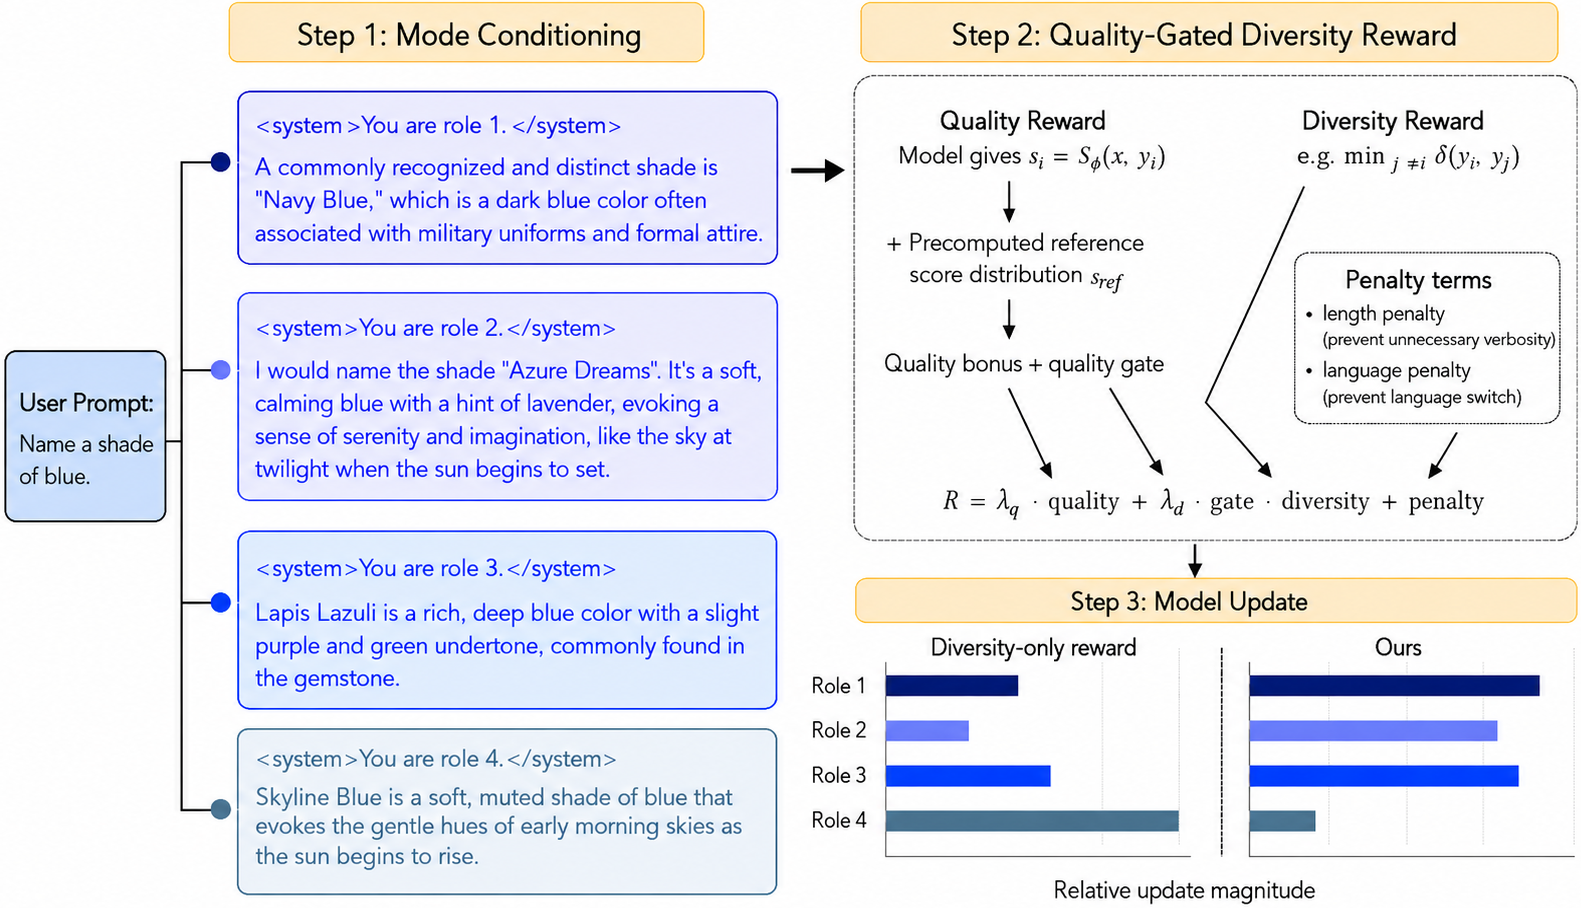
\includegraphics[width=\textwidth]{figures/method_v2.png}
        \label{fig:architecture}
    \end{subfigure}\hfill
    \begin{subfigure}[t]{0.2\linewidth}
        \centering
        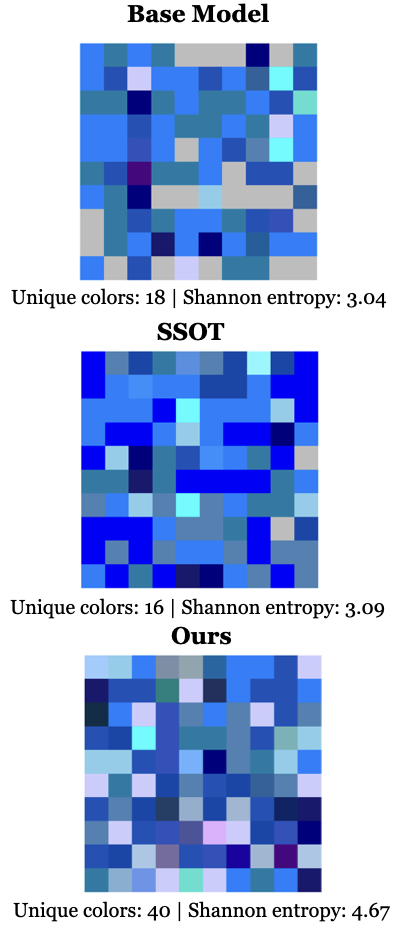
\includegraphics[width=\linewidth]{figures/blue.png}
        \label{fig:40blue}
    \end{subfigure}
    \vspace{-0.2cm}
\caption{Left: Overview of \method. \method~uses mode conditioning to elicit diverse candidate responses, then applies a quality gated diversity reward with penalty terms to promote high-quality diversity while suppressing low-quality or reward-hacking outputs. Right: 100 responses to the prompt \textbf{`Name a shade of blue''} from Qwen-3-8B (base), \ssot, and \method~under diverse mode inference. \method~produces 40 distinct shades of blue, 122\% more than the base model and 150\% more than \ssot, with 100\% valid answers, versus 20\% invalid answers from the base model. 
}
\label{fig:moda + 40blue}
\end{figure}

\section{Preliminaries: LLM Alignment with Reinforcement Learning}

% \liwei{talk about preliminary of LLM alignment with GRPO. And mention why it induce mode collapse -- bc it only incentivize the model to seek the highest reward region, without flexibility to accommodate more high reward outcomes.}

% \liwei{move the intro of reward to the next section}
Let $\mathcal{S}$ denote the set of natural language token sequences.
A language model $\pi(\cdot \mid x)$ takes a prompt $x \in \mathcal{S}$ as input and outputs a probability distribution over $\mathcal{S}$.
We denote the probability of a specific response $y \in \mathcal{S}$ as $\pi(y \mid x)$.
Given a prompt $x$, we sample $k$ independent responses
$\{y_1, y_2, \ldots, y_k\} \sim \pi(\cdot \mid x)$,
forming a \textit{response group} $\mathcal{Y} = \{y_i\}_{i=1}^{k}$. While RL post-training on LLMs demonstrates strong empirical results in enhancing reasoning capability\citep{shao2024deepseekmath, Guo_2025}, it is known to suffer from mode collapse. Conventional RL post-training only incentivizes the model to seek the highest reward region, without flexibility to accommodate more diverse responses. Our goal is to optimize the policy so that the generated responses are not only high-quality, but also diverse, creative, and non-redundant. 

%We therefore introduce \textbf{Quality-Gated Diversity Reward} which jointly values \textit{quality} and \textit{diversity} within the response group $\mathcal{Y}$ by gating the diversity term by quality to prevent the model from being rewarded for producing unusual but degenerate responses, described in Section \ref{subsec:qgdr}

% \liwei{this section is too short and hence a bit weird to keep it an independent section. can we fold it into current section 4, as the first subsection?}
